\documentclass[10pt,a4paper,final]{report}
\usepackage[utf8]{inputenc}
\usepackage[english]{babel}
\usepackage{amsmath}
\usepackage{amsfonts}
\usepackage{amssymb}
\usepackage{float}
\usepackage{fancyhdr}
\usepackage{enumitem}
\usepackage{graphicx}
\usepackage{listings}
\pagestyle{fancy}


\begin{document}
\lstset{language=SQL}
\chead{
Daniel S. Fridjonsson,
Lars Andersen,
S\o ren S. Als \&
Mathias W. Pedersen.
sw608f14 - Room: 2.1.10}


\section*{Self study 1 - miniproject part 1}
Actors, directors, and writers are decided to be stored only as person, since they can preform multiple roles throughout their career. A person has a name, birthday, and additional information. The table for persons will be:

\begin{table}[H] \centering
\begin{tabular}{|c|c|c|}
\hline 
PERSON ID & PERSON NAME & BIRTHDAY \\ 
\hline 
123 & Johnny Known & 03-09-1934 \\ 
\hline 
\end{tabular} 
\end{table}

A movie can contain movie name, movie id, release data, and rating. The rating is calculated by taking the average of the user ratings, see last table, for a specific movie.

\begin{table}[H] \centering
\begin{tabular}{|c|c|c|c|}
\hline 
MOVIE ID & MOVIE NAME & RELEASE DATE & RATING\\ 
\hline 
123 & The Hobbit & 05-12-2014 & 9.2\\ 
\hline 
\end{tabular} 
\end{table}

To connect persons to movies another table is used. Where the role in this table is an enum that contains actor, director, and writer.

\begin{table}[H] \centering
\begin{tabular}{|c|c|c|}
\hline 
MOVIE ID & PERSON ID & ROLE \\ 
\hline 
637 & 463 & Actor \\ 
\hline 
563 & 563 & Director \\ 
\hline 
637 & 674 & Writer \\ 
\hline 
\end{tabular}
\end{table}

Awards can be given to both persons and movies, therefore it is necessary to have two tables, since the id's can be the same for both persons and movies. The tables will be as follows:

\begin{table}[H] \centering
\begin{tabular}{|c|c|c|}
\hline 
MOVIE ID & AWARD & YEAR \\ 
\hline 
542 & Best Picture & 2013 \\ 
\hline 
\end{tabular} 
\end{table}

\begin{table}[H] \centering
\begin{tabular}{|c|c|c|c|}
\hline 
PERSON ID & MOVIE ID & AWARD & YEAR\\ 
\hline 
524 & 542 & Best Actor & 2013 \\ 
\hline 
\end{tabular} 
\end{table}

To store a user of the system it is necessary to store a username and password. The password should be encrypted, but security is not the focus of this exercise.

\begin{table}[H] \centering
\begin{tabular}{|c|c|c|}
\hline 
USER ID & USERNAME & PASSWORD \\ 
\hline 
546 & NiceName & 123456 \\ 
\hline 
\end{tabular} 
\end{table}

Furthermore, a user can rate movies, and a table for this is created. This table contains user id, movie id, and rating

\begin{table}[H] \centering
\begin{tabular}{|c|c|c|}
\hline 
MOVIE ID & USER ID & RATING \\ 
\hline 
634 & 342 & 8 \\ 
\hline 
\end{tabular} 
\end{table}
\newpage
\section*{Self study 2 - miniproject part 2}

\subsection*{ER Diagram}
\begin{figure}[H]
     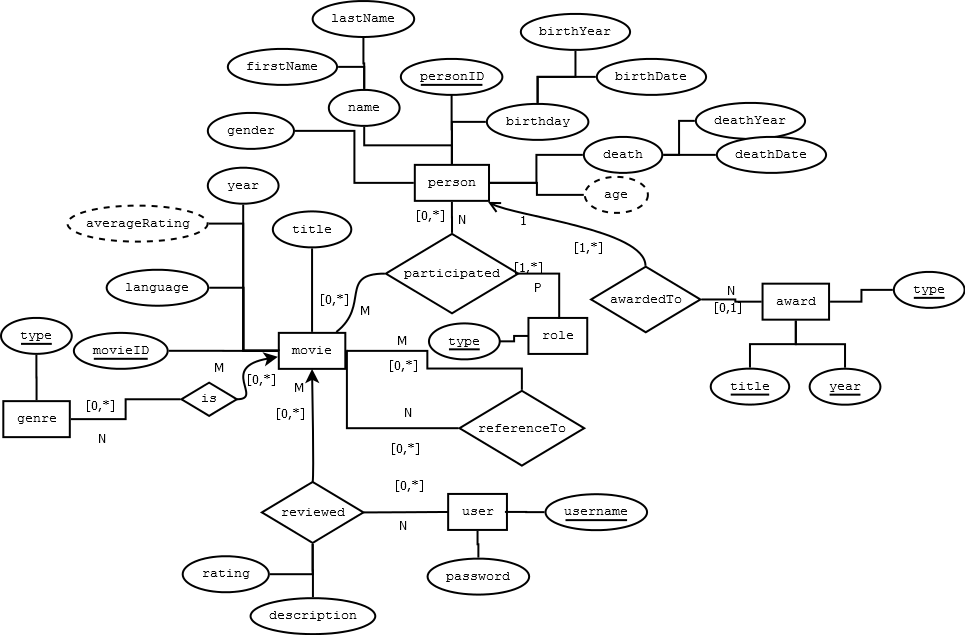
\includegraphics[scale=0.4]{ERdiagram.png}
     \caption{ER Diagram selfstudy 2}
\end{figure}
\subsection*{Relational Schema}
\begin{description}[style=nextline]
     \item[genre]
     $\{[\underline{type:String}]\}$
     \item[movie]
     $\{[\underline{movieID:Int},language:String,year:Int,title:String]\}$
     \item[user]
     $\{[\underline{username:String},password:String]\}$
     \item[award]
     $\{[\underline{title:String, year:Int, type:String}, receiver \rightarrow person]\}$
     \item[person]
     $\{[\underline{personID:Int},firstName:String, lastName:String, gender:String, birthYear:Int, birthDate:String, deathYear:Int, deathDate:String]\}$
     \item[participated]
     $\{[\underline{movieID\rightarrow movie, personID \rightarrow person, type \rightarrow role}]\}$
     \item[is]
     $\{[\underline{type \rightarrow genre, movieID \rightarrow movie}]\}$
     \item[reviewed]
     $\{[\underline{movieID \rightarrow movie, username \rightarrow user}, rating:Int, description:String]\}$
     \item[referenceTo]
     $\{[\underline{from \rightarrow movie, to \rightarrow movie}]\}$
\end{description}

\subsection*{Reflections}
The design is different from the initial design in that the initial design was at a mere table level. Furthermore, several additional attributes have been added to accommodate the expected information requirements.
Another change is that there was no primary and foreign keys highlighted in the original answer.
Average rating in the initial database was intended to be a calculated attribute, but was not listed as such, contrary to the new design.
Additionally we have decided that an award only can be given to a person, as that made the design simpler.
Finally we added the $referenceTo$ relation, as that was a requirement we missed in the first selfstudy.


\section*{Selfstudy 4}
\subsection*{Revised ER Diagram}
\begin{figure}[H]
     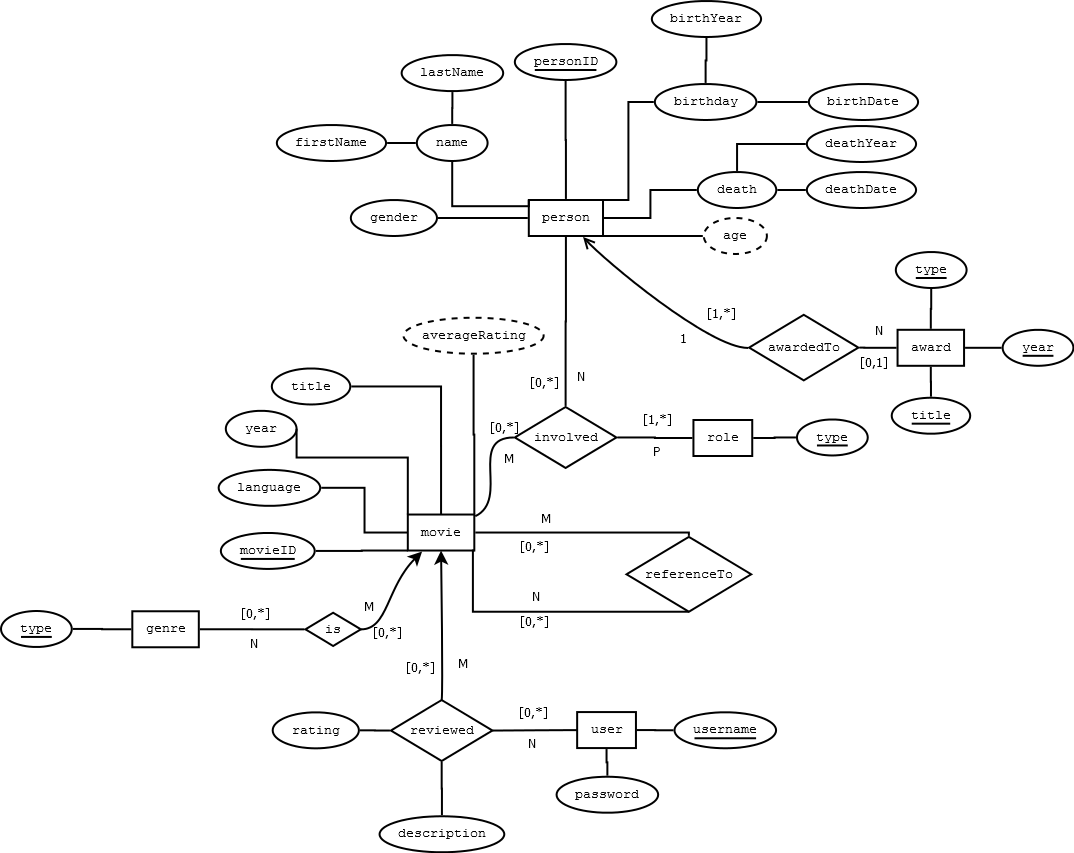
\includegraphics[scale=0.4]{ERdiagramrevisioned}
     \caption{Revised ER Diagram selfstudy 4}
\end{figure}
\subsection*{Revised relational schema}
\subsection*{ER Diagram}
\begin{figure}[h]
     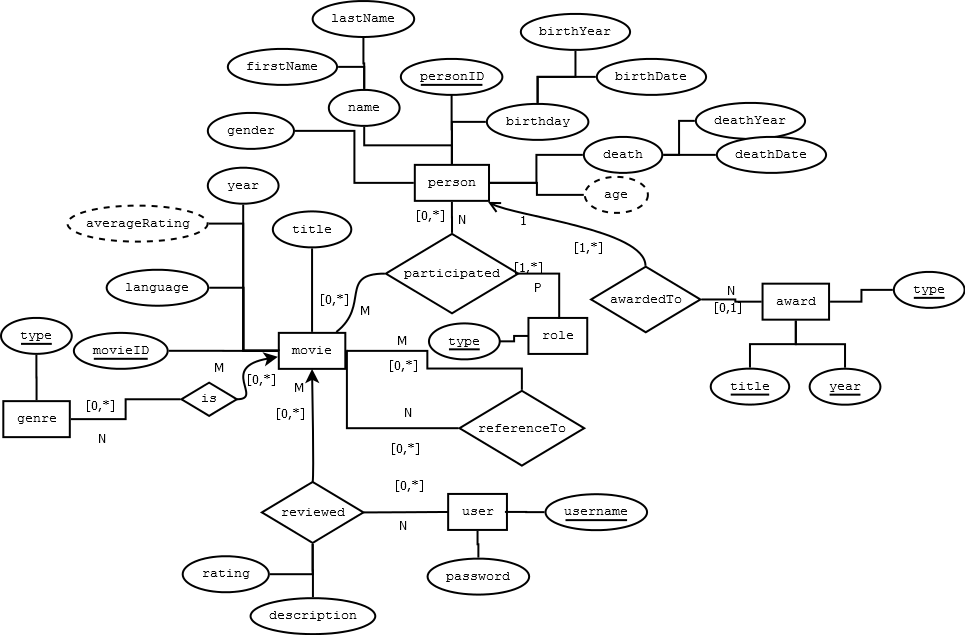
\includegraphics[scale=0.4]{ERdiagram.png}
\end{figure}
\subsection*{Relational Schema}
\begin{description}[style=nextline]
     \item[genre]
     $\{[\underline{type:String}]\}$
     \item[role]
     $\{[\underline{type:String}]\}$
     \item[movie]
     $\{[\underline{movieID:Int},language:String,year:Int,title:String]\}$
     \item[user]
     $\{[\underline{username:String},password:String]\}$
     \item[award]
     $\{[\underline{title:String, year:Int, type:String}, receiver:Int \rightarrow person]\}$
     \item[person]
     $\{[\underline{personID:Int},firstName:String, lastName:String, gender:String, birthYear:Int, birthDate:String, deathYear:Int, deathDate:String]\}$
     \item[involved]
     $\{[\underline{movieID:Int\rightarrow movie, personID:Int \rightarrow person, type:String \rightarrow role}]\}$
     \item[is]
     $\{[\underline{type:String \rightarrow genre, movieID:Int \rightarrow movie}]\}$
     \item[reviewed]
     $\{[\underline{movieID:Int \rightarrow movie, username:String \rightarrow user}, rating:Int, description:String]\}$
     \item[referenceTo]
     $\{[\underline{from:Int \rightarrow movie, to:Int \rightarrow movie}]\}$
\end{description}

\subsection*{Functional Dependencies}

\begin{equation*}
\begin{aligned}
     genre.type &\rightarrow Ø \\
     role.type &\rightarrow Ø \\
     movieID &\rightarrow language, movie.year, movie.title\\
     username  &\rightarrow password \\
     award.title, award.year, award.type &\rightarrow  personID\\
     personID &\rightarrow firstName, lastName, gender, birthYear, birthDate, deathYear, deathDate \\
     movieID, personID, role.type &\rightarrow  Ø \\
     genre.type, movieID &\rightarrow Ø \\     
     movieID, username &\rightarrow rating, description\\
     movieID, movieID &\rightarrow Ø
\end{aligned}
\end{equation*}

It is 3NF as rule 2 applies for all the functional dependencies, since the primary key in each relation is also a super key and due to it being 2NF, as it is fully functionally dependent.
As it is rule 2 that applies for all the functional dependencies, it is also BCNF.

As the schema is already 3NF, there is no need to normalize the relations.

\subsection*{SQL Statements}
\begin{lstlisting}
CREATE TABLE genre
{
     type varchar(15) PRIMARY KEY
};

CREATE TABLE role
{
     type varchar(15) PRIMARY KEY
};


CREATE SEQUENCE serialmovie START 0;

CREATE TABLE movie
{
     movieID integer PRIMARY KEY DEFAULT nextval('serialmovie'),
     language varchar(20) DEFAULT 'English',
     year integer NOT NULL,
     title varchar(100) NOT NULL
};

CREATE TABLE user
{
     username varchar(20) PRIMARY KEY,
     password varchar(50) NOT NULL
};

CREATE TABLE award
{
     title varchar(30),
     year integer,
     type varchar(15),
     receiver integer NOT NULL,
     PRIMARY KEY(title,year,type),
     FOREIGN KEY(receiver) REFERENCES person(personID)
};

CREATE SEQUENCE serialperson START 0;

CREATE TABLE person
{
     personID integer PRIMARY KEY DEFAULT nextval('serialperson'),
     firstName varchar(20) NOT NULL,
     lastName varchar(50) NOT NULL,
     gender varchar(6),
     birthYear integer,
     birthDate varchar(7),
     deathYear integer,
     deathDate varchar(7)
};

CREATE TABLE involved
{
     movieID integer,
     personID integer,
     type varchar(15),
     PRIMARY KEY(movieID, personID, type),
     FOREIGN KEY(movieID) REFERENCES movie(movieID),
     FOREIGN KEY(personID) REFERENCES person(personID),
     FOREIGN KEY(type) REFERENCES role(type)
}

CREATE TABLE is
{
     type varchar(15),
     movieID integer,
     PRIMARY KEY(type,movieID),
     FOREIGN KEY(type) REFERENCES genre(type),
     FOREIGN KEY(movieID) REFERENCES movie(movieID)
};

CREATE TABLE reviewed
{
     movieID integer,
     username varchar(20),
     rating integer NOT NULL,
     description varchar(MAX),
     PRIMARY KEY(movieID, username),
     FOREIGN KEY(movieID) REFERENCES movie(movieID),
     FOREIGN KEY(username) REFERENCES user(username)
};

CREATE TABLE referenceTo
{
     from integer,
     to integer,
     PRIMARY KEY(from, to),
     FOREIGN KEY(from,to) REFERENCES movie(movieID)
};
\end{lstlisting}

\subsection*{Reflections}
Differences from the original design is that we changed the layout of our ER Diagram and renamed the \textit{participated} relation to \textit{involved}.
Considerations we have to take in the future is our encoding of dates, which could be changed to the \textit{DATETIME} datatype.
Also, we forgot the role relation in our first schema, and was thus added to the revised schema.

\section*{Selfstudy 5}
\subsection*{Setup of the Database}
We already provided the given sql statements for setting up our database, however, some slight modifications were performed.
Curly brackets were changed to ordinary parentheses.
Additionally to better fit the imdb data, the following was changed:
\begin{itemize}
     \item Removed birthyear and deathyear, so it was included in birthdate and deathdate
     \item Made birthdate and deathdate 20 in size
     \item Merged firstname and lastname into name
     \item Made name 500 in size (there was some really long names)
     \item Title of movie changed to 500 length
\end{itemize}

Here is the new table creation commands:
\begin{lstlisting}{language = SQL}
CREATE TABLE genre
(
     type varchar(15) PRIMARY KEY
);

CREATE TABLE role
(
     type varchar(15) PRIMARY KEY
);


CREATE SEQUENCE serialmovie START 1;

CREATE TABLE movie
(
     movieID integer PRIMARY KEY DEFAULT nextval('serialmovie'),
     language varchar(50) DEFAULT 'English',
     year integer NOT NULL,
     title varchar(500) NOT NULL
);

CREATE TABLE users
(
     username varchar(20) PRIMARY KEY,
     password varchar(50) NOT NULL
);

CREATE SEQUENCE serialperson START 1;

CREATE TABLE person
(
     personID integer PRIMARY KEY DEFAULT nextval('serialperson'),
     name varchar(500) NOT NULL,
     gender varchar(6),
     birthDate varchar(20),
     deathDate varchar(20)
);

CREATE TABLE award
(
     title varchar(30),
     year integer,
     type varchar(15),
     receiver integer NOT NULL,
     PRIMARY KEY(title,year,type),
     FOREIGN KEY(receiver) REFERENCES person(personID)
);


CREATE TABLE involved
(
     movieID integer,
     personID integer,
     type varchar(15),
     PRIMARY KEY(movieID, personID, type),
     FOREIGN KEY(movieID) REFERENCES movie(movieID),
     FOREIGN KEY(personID) REFERENCES person(personID),
     FOREIGN KEY(type) REFERENCES role(type)
);

CREATE TABLE isA
(
     type varchar(15),
     movieID integer,
     PRIMARY KEY(type,movieID),
     FOREIGN KEY(type) REFERENCES genre(type),
     FOREIGN KEY(movieID) REFERENCES movie(movieID)
);

CREATE TABLE reviewed
(
     movieID integer,
     username varchar(20),
     rating integer NOT NULL,
     description text,
     PRIMARY KEY(movieID, username),
     FOREIGN KEY(movieID) REFERENCES movie(movieID),
     FOREIGN KEY(username) REFERENCES users(username)
);

CREATE TABLE referenceTo
(
     froma integer,
     toa integer,
     PRIMARY KEY(froma, toa),
     FOREIGN KEY(froma) REFERENCES movie(movieID),
     FOREIGN KEY(toa) REFERENCES movie(movieID)
);
\end{lstlisting}
\subsection*{Modifications to imdb dump}
\begin{itemize}
     \item int to integer
     \item removed \lstinline!ENGINE=InnoDB DEFAULT CHARSET=latin1;!
     \item Changed indexes from \lstinline!KEY idx5 (movieId,genre)! 
     \item[] to \lstinline!CREATE INDEX idx5 ON genre (movieId, genre);! and similar for the other indexes.
     \item keywords like \textit{user} was changed to \textit{\"user\"} as it was a keyword.
     \item ' was changed to ''
\end{itemize}

\subsection*{Importing Data from IMDB\_db to our Database}
In general we used a copy command to copy the desired data fra IMDB\_db to a .csv file and then copying that information to our database.
Also, sorry for a lot of commands :).
\subsubsection*{genre}
\textbf{To csv file}
\begin{lstlisting}
psql -d IMDB_db -U postgres 
-c "\COPY (SELECT DISTINCT genre.genre as type FROM genre)
\end{lstlisting}
\textbf{To our database}
\begin{lstlisting}
psql -d ourmovieDB -U postgres 
-c "\COPY genre(type) FROM 'PATH\genre.csv'
\end{lstlisting}

\subsubsection*{person}
\textbf{To csv file}
\begin{lstlisting}
psql -d IMDB_db -U postgres 
-c "\COPY (SELECT DISTINCT id, name, gender, birthdate, deathdate FROM person) 
To 'PATH\person.csv'"
\end{lstlisting}

\textbf{To our database}
\begin{lstlisting}
psql -d ourmovieDB -U postgres 
-c "\COPY person(personID,name,gender,birthDate,deathDate) 
FROM 'PATH\person.csv'"
\end{lstlisting}

\subsubsection*{role}
\textbf{To csv file}
\begin{lstlisting}
psql -d IMDB_db -U postgres 
-c "\COPY (SELECT DISTINCT role FROM involved) 
To 'PATH\role.csv'"
\end{lstlisting}
\textbf{To our database}
\begin{lstlisting}
psql -d ourmovieDB -U postgres 
-c "\COPY role(type) 
FROM 'PATH\role.csv'"
\end{lstlisting}

\subsubsection*{movie}
\textbf{To csv file}
\begin{lstlisting}
psql -d IMDB_db -U postgres 
-c "\COPY (SELECT DISTINCT id, language, year, title 
FROM movie) To 'PATH\movie.csv'"
\end{lstlisting}
\textbf{To our database}
\begin{lstlisting}
psql -d ourmovieDB -U postgres 
-c "\COPY movie(movieID, language, year, title) 
FROM 'PATH\movie.csv'"
\end{lstlisting}

\subsubsection*{danishmovies $\rightarrow$ movie}
\textbf{To csv file}
\begin{lstlisting}
psql -d IMDB_db -U postgres 
-c "\COPY (SELECT DISTINCT 'Danish', year, title FROM danishmovies) 
To 'PATH\danishmovie.csv'"
\end{lstlisting}
\textbf{To our database}
\begin{lstlisting}
psql -d ourmovieDB -U postgres 
-c "\COPY movie(language, year, title) 
FROM 'PATH\danishmovie.csv'"
\end{lstlisting}

\subsubsection*{referenceTo}
\textbf{To csv file}
\begin{lstlisting}
psql -d IMDB_db -U postgres 
-c "\COPY (SELECT DISTINCT fromid, toid FROM movieref) 
To 'PATH\referemceto.csv'"
\end{lstlisting}
\textbf{To our database}
\begin{lstlisting}
psql -d ourmovieDB -U postgres 
-c "\COPY referenceTo(froma,toa) 
FROM 'PATH\referemceto.csv'"
\end{lstlisting}

\subsubsection*{involved - part1}
\textbf{To csv file}
\begin{lstlisting}
psql -d IMDB_db -U postgres 
-c "\COPY (SELECT DISTINCT movieid, personid, role FROM involved) 
To 'PATH\involved.csv'"
\end{lstlisting}
\textbf{To our database}
\begin{lstlisting}
psql -d ourmovieDB -U postgres 
-c "\COPY involved(movieID,personID,type) 
FROM 'PATH\involved.csv'"
\end{lstlisting}

\subsubsection*{involved - part1 get directors from danishmovies}
We found that postgres does not allow queries over multiple databases. As a solution we made a wrapper table in our database.
\begin{lstlisting}
        CREATE TABLE wrapperdanishdirector(
            title varchar(500) NOT NULL,
            director varchar(500) NOT NULL,
        );
\end{lstlisting}

\textbf{To csv file}
\begin{lstlisting}
psql -d IMDB_db -U postgres 
-c "\COPY (SELECT DISTINCT title, director FROM danishmovies) 
To 'PATH\involvedwrapper.csv'"
\end{lstlisting}
\textbf{To our database - in wrapper table}
\begin{lstlisting}
psql -d ourmovieDB -U postgres 
-c "\COPY wrapperdanishdirector(title,director) 
FROM 'PATH\involvedwrapper.csv'"
\end{lstlisting}

\textbf{Adding to involved table}
\begin{lstlisting}
INSERT INTO involved SELECT DISTINCT movie.movieID, person.personID,'director' 
FROM movie, wrapperdanishdirector, person 
WHERE movie.title = wrapperdanishdirector.title 
AND wrapperdanishdirector.director = person.name 
AND (movie.movieID, person.personID,'director') NOT IN (SELECT * 
FROM involved)
\end{lstlisting}

\subsubsection*{users}
\textbf{To csv file}
\begin{lstlisting}
psql -d IMDB_db -U postgres 
-c "\COPY (SELECT DISTINCT ratings.user, '1234' FROM ratings) 
To 'PATH\users.csv'"
\end{lstlisting}
\textbf{To our database}
\begin{lstlisting}
psql -d ourmovieDB -U postgres 
-c "\COPY users(username,password) 
FROM 'PATH\users.csv'"
\end{lstlisting}

\subsubsection*{isa}
\textbf{To csv file}
\begin{lstlisting}
psql -d IMDB_db -U postgres 
-c "\COPY (SELECT DISTINCT genre.genre, movieid FROM genre) 
To 'PATH\is.csv'"
\end{lstlisting}
\textbf{To our database}
\begin{lstlisting}
psql -d ourmovieDB -U postgres 
-c "\COPY isa(type, movieid) 
FROM 'PATH\is.csv'"
\end{lstlisting}

\subsubsection*{reviewed}
It seemed like some movies that was reviewed was not part of the set of movies from the imdb database. For that reason we made a temp reviewed table:
\begin{lstlisting}
CREATE TABLE tempreviewed(
     movieID integer,
     username varchar(20),
     rating integer NOT NULL
);
\end{lstlisting}
\textbf{To csv file}
\begin{lstlisting}
psql -d IMDB_db -U postgres 
-c "\COPY (SELECT DISTINCT movieid, ratings.user, rating  FROM ratings) 
To 'PATH\reviewed.csv'"
\end{lstlisting}
\textbf{To our tempreviewed table in database}
\begin{lstlisting}
psql -d ourmovieDB -U postgres 
-c "\COPY tempreviewed(movieid, username, rating) 
FROM 'PATH\reviewed.csv'"
\end{lstlisting}
\textbf{Final insertion into reviewed table}
\begin{lstlisting}
INSERT INTO reviewed SELECT * FROM tempreviewed 
WHERE tempreviewed.movieid IN (SELECT DISTINCT movieid from movie)
\end{lstlisting}
\subsection*{SQL Statements and results}

\subsubsection*{1.}
\textbf{Query:}
\begin{lstlisting}
SELECT count(*) FROM movie WHERE language = 'Danish';
\end{lstlisting}
\textbf{Result:}\\
670

\subsubsection*{2.}
\textbf{Query:}
\begin{lstlisting}
SELECT year, count(reviewed.rating) FROM movie,reviewed 
WHERE movie.movieID = reviewed.movieID GROUP BY year;
\end{lstlisting}

\textbf{Result:}

\begin{tabular}{|c|c|}
\hline 
2000 & 24 \\ 
\hline 
1962 & 1 \\ 
\hline 
2007 & 25 \\ 
\hline 
2002 & 19 \\ 
\hline 
1992 & 3 \\ 
\hline 
2008 & 40 \\ 
\hline 
2003 & 27 \\ 
\hline 
1999 & 48 \\ 
\hline 
2005 & 30 \\ 
\hline 
2004 & 13 \\ 
\hline 
\end{tabular} 

\subsubsection*{3..}
\textbf{Query:}
\begin{lstlisting}
SELECT title FROM movie WHERE movieID IN 
   (SELECT i1.movieID FROM involved i1, involved i2 
   WHERE i1.movieID = i2.movieID AND i1.personID IN 
   (SELECT personID FROM person WHERE name = 'John Travolta') 
    AND i2.personID IN (SELECT personID FROM person WHERE name = 'Uma Thurman') 
    AND i1.type = 'actor' AND i2.type = 'actor');
\end{lstlisting}
\textbf{Result:}

\begin{tabular}{|c|}
\hline 
Good Morning America \\ 
\hline 
The Rosie O'Donnell Show \\ 
\hline 
The Oprah Winfrey Show \\
\hline
The View \\ 
\hline 
Wetten, dass..? \\ 
\hline 
Late Show with David Letterman \\ 
\hline 
The Tonight  Show with Jay Leno \\ 
\hline 
You're Still Not Fooling Anybody \\ 
\hline 
HBO First Look \\ 
\hline 
Boffo! Tinseltown's Bombs and Blockbusters \\
\hline 
\end{tabular} 

\subsubsection*{4.}
\textbf{Query:}
\begin{lstlisting}
SELECT count(*) FROM person WHERE personID IN (SELECT DISTINCT personID 
FROM involved WHERE type = 'actor' OR type = 'director') AND name LIKE 'Q%';
\end{lstlisting}
\textbf{Result:}
153

\subsubsection*{5.}
\textbf{Query:}
\begin{lstlisting}
SELECT count(*) FROM (SELECT username FROM reviewed 
GROUP BY username HAVING count(movieID) >= 3) as alias;
\end{lstlisting}
\textbf{Result:}\\
34
\subsubsection*{6.}
\textbf{Query:}
\begin{lstlisting}
SELECT name, substring(birthdate from 1 for 4) FROM person 
WHERE personID IN (SELECT personID FROM involved WHERE movieID 
IN (SELECT movieID FROM movie WHERE title = 'Pulp Fiction') AND type = 'actor') 
ORDER BY birthdate ASC;
\end{lstlisting}
\textbf{Result:}

\begin{tabular}{|c|c|}
\hline 
Emil Sitka & 1914 \\ 
\hline 
Harvey Keitel & 1939 \\ 
\hline 
Rene Beard & 1941 \\ 
\hline 
Christopher Walken & 1943 \\ 
\hline 
Joseph Pilato & 1949 \\ 
\hline 
Brenda Hillhouse & 1953 \\ 
\hline 
John Travolta & 1954 \\ 
\hline 
Bruce Willis & 1955 \\ 
\hline 
Amanda Plummer & 1957 \\ 
\hline 
Lawrence Bender & 1957 \\ 
\hline 
\end{tabular} 

\subsubsection*{7.}
\textbf{Query:}
\begin{lstlisting}
SELECT title, year FROM movie WHERE movieID IN 
(SELECT movieID FROM involved WHERE personID IN 
   (SELECT personID FROM person WHERE name = 'John Travolta') 
   AND type ='actor') AND year >= 1980 AND year < 1990;
\end{lstlisting}
\textbf{Result:}

\begin{tabular}{|c|c|}
\hline Wetten, dass..? & 1981 \\ 
\hline Larry King Live & 1985 \\ 
\hline That's Dancing! & 1985 \\ 
\hline Perfect & 1985 \\ 
\hline Biography & 1987 \\ 
\hline Two of a Kind & 1983 \\ 
\hline Staying Alive & 1983 \\ 
\hline Live with Regis and Kathie Lee & 1988 \\ 
\hline Entertainment Tonight & 1981 \\ 
\hline Urban Cowboy & 1980 \\ 
\hline 
\end{tabular}

\subsubsection*{8.}
\textbf{Query:}
\begin{lstlisting}
SELECT title FROM movie WHERE movieID IN 
   (SELECT movieID FROM reviewed GROUP BY movieID ORDER BY AVG(rating) 
      DESC) 
   AND year >= 1990 AND year < 2000 LIMIT 2;
\end{lstlisting}
\textbf{Result:}\\
The Usual Suspects\\
The Shawshank Redemption
\subsubsection*{9.}
\textbf{Query:}
\begin{lstlisting}
SELECT title FROM movie WHERE movieID IN 
   (SELECT movieID FROM reviewed WHERE movieID IN 
      (SELECT movieID FROM reviewed 
      GROUP BY movieID HAVING count(rating) >= 2) 
   GROUP BY movieID ORDER BY AVG(rating) DESC )  
AND year >= 1990 AND year < 2000 LIMIT 2;
\end{lstlisting}
\textbf{Result:}\\
The Usual Suspects\\
The Shawshank Redemption

\subsubsection*{10.}
\textbf{Query:}
\begin{lstlisting}
SELECT language, AVG(rating) FROM reviewed, movie 
WHERE reviewed.movieID = movie.movieID AND year = 1994 GROUP BY language
\end{lstlisting}
\textbf{Result:}

\begin{tabular}{|c|c|}
\hline 
NULL & 7.0 \\ 
\hline 
French & 9.0 \\ 
\hline 
English & 8.304 \\ 
\hline 
\end{tabular} 

\subsubsection*{11.}
\textbf{Query:}
\begin{lstlisting}
SELECT name FROM person WHERE personID IN 
   (SELECT AVG(personID) FROM involved WHERE personID in 
      (SELECT personID FROM involved WHERE movieID in 
         (SELECT movieID FROM movie WHERE title = 'Pulp Fiction') 
       AND type = 'actor') 
GROUP BY movieID HAVING count(personID) = 1);
\end{lstlisting}
\textbf{Result:}

\begin{tabular}{|c|}
\hline 
Caleb Allen \\ 
\hline 
Rosana Arquette \\ 
\hline 
Steve Buscemi \\ 
\hline 
Maria de Medeiros \\ 
\hline 
Karen Maruyama \\ 
\hline 
Burr Steers \\ 
\hline 
Eric Stoltz \\ 
\hline 
Julia Sweeney \\ 
\hline 
Quentin Tarantino \\ 
\hline 
Christopher Walken \\ 
\hline 
\end{tabular} 

\subsubsection*{12.}
\textbf{Query:}
\begin{lstlisting}
SELECT title FROM movie WHERE movieID IN 
   (SELECT movieID FROM reviewed WHERE movieID IN 
      (SELECT movie.movieID FROM movie,involved, person 
      WHERE name = 'John Travolta' 
      AND person.personID = involved.personID AND type = 'actor' 
      AND movie.movieID = involved.movieID) 
GROUP BY movieID ORDER BY AVG(rating) DESC LIMIT 1);
\end{lstlisting}
\textbf{Result:}

Pulp Fiction

\subsubsection*{13.}
\textbf{Query:}
\begin{lstlisting}
SELECT count(*)FROM person p1, person p2 WHERE p1.personID IN 
(SELECT personID FROM involved WHERE type = 'actor') 
AND p2.name = 'Charles Chaplin' AND p1.gender='f'
AND (p1.birthdate > p2.deathdate 
OR p2.birthdate > p1.deathdate);
\end{lstlisting}
\textbf{Result:}

5405

\subsubsection*{14.}
\textbf{Query:}
\begin{lstlisting}
SELECT type,AVG(rating) FROM isa, reviewed 
WHERE isa.movieID = reviewed.movieID GROUP BY type;
\end{lstlisting}
\textbf{Result:}

\begin{tabular}{|c|c|}
\hline 
Comedy & 7.2381 \\ 
\hline 
Drama & 7.8333 \\ 
\hline 
Fantasy & 7.2430 \\ 
\hline 
Biography & 8.1333 \\ 
\hline 
Thriller & 7.7824 \\ 
\hline 
Crime & 8.3950 \\ 
\hline 
Muscial & 7 \\ 
\hline 
War & 8.692 \\ 
\hline 
History & 8.1250 \\ 
\hline 
Adventure & 7.4211 \\ 
\hline 
\end{tabular} 

\subsubsection*{15.}
\textbf{Query:}
\begin{lstlisting}
SELECT type,AVG(rating) FROM isa, reviewed 
WHERE isa.movieID = reviewed.movieID 
GROUP BY type HAVING count(rating) >= 2;
\end{lstlisting}
\textbf{Result:}

\begin{tabular}{|c|c|}
\hline Comedy & 7.2381 \\ 
\hline Drama & 7.8333 \\ 
\hline Fantasy & 7.2430 \\ 
\hline Biography & 8.1333 \\ 
\hline Thriller & 7.7824 \\ 
\hline Crime & 8.3950 \\ 
\hline War & 8.2692 \\ 
\hline History & 8.1250 \\ 
\hline Adventure & 7.4211 \\ 
\hline Sci-Fi & 7.4853 \\ 
\hline 
\end{tabular}
\subsubsection*{16.}
\textbf{Query:}
\begin{lstlisting}
SELECT title FROM movie 
WHERE movieID IN 
   (SELECT r1.froma FROM referenceTo r1, referenceTo r2
      WHERE r1.toa = r2.froma 
      GROUP BY r1.froma ORDER BY count(r2.toa) DESC LIMIT 1);
\end{lstlisting}
\textbf{Result:}\\
Saturday Night Live
\subsubsection*{17.}
\textbf{Query:}
\begin{lstlisting}
SELECT count(foo.personID) FROM 
   (SELECT DISTINCT i1.personID FROM involved i1, involved i2 
   WHERE i1.personID = i2.personID AND i1.type = 'actor' 
      AND i2.type = 'director') AS foo;
\end{lstlisting}
\textbf{Result:}\\
5930
\subsubsection*{18.}
\textbf{Query:}
\begin{lstlisting}
SELECT i1.type,i2.type FROM isa i1, isa i2 
WHERE i1.type != i2.type AND i1.movieID = i2.movieID 
GROUP BY i1.type, i2.type ORDER BY count(i1.movieID) DESC LIMIT 1;
\end{lstlisting}
\textbf{Result:}

\begin{tabular}{|c|c|}
\hline 
Romance & Drama \\ 
\hline 
\end{tabular} 
\end{document}
